\documentclass[12pt,a4paper]{article}

%%%%%%%%------------------------------------------------------------------------
%%%% 日常所用宏包

%% 控制页边距
% 如果是beamer文档类, 则不用geometry
\makeatletter
\@ifclassloaded{beamer}{}{\usepackage[top=2.5cm, bottom=2.5cm, left=2.5cm, right=2.5cm]{geometry}}
\makeatother

%% 控制项目列表
\usepackage{enumerate}

%% 多栏显示
\usepackage{multicol}

%% 算法环境
\usepackage{algorithm}  
\usepackage{algorithmic} 
\usepackage{float} 

%% 网址引用
\usepackage{url}

%% 控制矩阵行距
\renewcommand\arraystretch{1.4}

%% hyperref宏包,生成可定位点击的超链接,并且会生成pdf书签
\makeatletter
\@ifclassloaded{beamer}{
\usepackage{hyperref}
}{
\usepackage[%
    pdfstartview=FitH,%
    CJKbookmarks=true,%
    bookmarks=true,%
    bookmarksnumbered=true,%
    bookmarksopen=true,%
    colorlinks=true,%
    citecolor=blue,%
    linkcolor=blue,%
    anchorcolor=green,%
    urlcolor=blue%
]{hyperref}
}
\makeatother



\makeatletter % 如果是 beamer 不需要下面两个包
\@ifclassloaded{beamer}{

}{
%% 控制标题
\usepackage{titlesec}
%% 控制目录
\usepackage{titletoc}
}
\makeatother

%% 控制表格样式
\usepackage{booktabs}

%% 控制字体大小
\usepackage{type1cm}

%% 首行缩进,用\noindent取消某段缩进
\usepackage{indentfirst}

%% 支持彩色文本、底色、文本框等
\usepackage{color,xcolor}

%% AMS LaTeX宏包: http://zzg34b.w3.c361.com/package/maths.htm#amssymb
\usepackage{amsmath,amssymb}

%%%% 基本插图方法
%% 图形宏包
\usepackage{graphicx}

%% 多个图形并排
\usepackage{subfig}

%%%% 基本插图方法结束

%%%% pgf/tikz绘图宏包设置
\usepackage{pgf,tikz}
\usetikzlibrary{shapes,automata,snakes,backgrounds,arrows}
\usetikzlibrary{mindmap}
%% 可以直接在latex文档中使用graphviz/dot语言,
%% 也可以用dot2tex工具将dot文件转换成tex文件再include进来
%% \usepackage[shell,pgf,outputdir={docgraphs/}]{dot2texi}
%%%% pgf/tikz设置结束


\makeatletter % 如果是 beamer 不需要下面两个包
\@ifclassloaded{beamer}{

}{
%%%% fancyhdr设置页眉页脚
%% 页眉页脚宏包
\usepackage{fancyhdr}
%% 页眉页脚风格
\pagestyle{plain}
}

%% 有时会出现\headheight too small的warning
\setlength{\headheight}{15pt}

%% 清空当前页眉页脚的默认设置
%\fancyhf{}
%%%% fancyhdr设置结束


\makeatletter % 对 beamer 要重新设置
\@ifclassloaded{beamer}{

}{
%%%% 设置listings宏包用来粘贴源代码
%% 方便粘贴源代码,部分代码高亮功能
\usepackage{listings}

%% 设置listings宏包的一些全局样式
%% 参考http://hi.baidu.com/shawpinlee/blog/item/9ec431cbae28e41cbe09e6e4.html
\lstset{
showstringspaces=false,              %% 设定是否显示代码之间的空格符号
numbers=left,                        %% 在左边显示行号
numberstyle=\tiny,                   %% 设定行号字体的大小
basicstyle=\footnotesize,                    %% 设定字体大小\tiny, \small, \Large等等
keywordstyle=\color{blue!70}, commentstyle=\color{red!50!green!50!blue!50},
                                     %% 关键字高亮
frame=shadowbox,                     %% 给代码加框
rulesepcolor=\color{red!20!green!20!blue!20},
escapechar=`,                        %% 中文逃逸字符,用于中英混排
xleftmargin=2em,xrightmargin=2em, aboveskip=1em,
breaklines,                          %% 这条命令可以让LaTeX自动将长的代码行换行排版
extendedchars=false                  %% 这一条命令可以解决代码跨页时,章节标题,页眉等汉字不显示的问题
}}
\makeatother
%%%% listings宏包设置结束


%%%% 附录设置
\makeatletter % 对 beamer 要重新设置
\@ifclassloaded{beamer}{

}{
\usepackage[title,titletoc,header]{appendix}
}
\makeatother
%%%% 附录设置结束


%%%% 日常宏包设置结束
%%%%%%%%------------------------------------------------------------------------


%%%%%%%%------------------------------------------------------------------------
%%%% 英文字体设置结束
%% 这里可以加入自己的英文字体设置
%%%%%%%%------------------------------------------------------------------------

%%%%%%%%------------------------------------------------------------------------
%%%% 设置常用字体字号,与MS Word相对应

%% 一号, 1.4倍行距
\newcommand{\yihao}{\fontsize{26pt}{36pt}\selectfont}
%% 二号, 1.25倍行距
\newcommand{\erhao}{\fontsize{22pt}{28pt}\selectfont}
%% 小二, 单倍行距
\newcommand{\xiaoer}{\fontsize{18pt}{18pt}\selectfont}
%% 三号, 1.5倍行距
\newcommand{\sanhao}{\fontsize{16pt}{24pt}\selectfont}
%% 小三, 1.5倍行距
\newcommand{\xiaosan}{\fontsize{15pt}{22pt}\selectfont}
%% 四号, 1.5倍行距
\newcommand{\sihao}{\fontsize{14pt}{21pt}\selectfont}
%% 半四, 1.5倍行距
\newcommand{\bansi}{\fontsize{13pt}{19.5pt}\selectfont}
%% 小四, 1.5倍行距
\newcommand{\xiaosi}{\fontsize{12pt}{18pt}\selectfont}
%% 大五, 单倍行距
\newcommand{\dawu}{\fontsize{11pt}{11pt}\selectfont}
%% 五号, 单倍行距
\newcommand{\wuhao}{\fontsize{10.5pt}{10.5pt}\selectfont}
%%%%%%%%------------------------------------------------------------------------


%% 设定段间距
\setlength{\parskip}{0.5\baselineskip}

%% 设定行距
\linespread{1}


%% 设定正文字体大小
% \renewcommand{\normalsize}{\sihao}

%制作水印
\RequirePackage{draftcopy}
\draftcopyName{XTUMESH}{100}
\draftcopySetGrey{0.90}
\draftcopyPageTransform{40 rotate}
\draftcopyPageX{350}
\draftcopyPageY{80}

%%%% 个性设置结束
%%%%%%%%------------------------------------------------------------------------


%%%%%%%%------------------------------------------------------------------------
%%%% bibtex设置

%% 设定参考文献显示风格
% 下面是几种常见的样式
% * plain: 按字母的顺序排列,比较次序为作者、年度和标题
% * unsrt: 样式同plain,只是按照引用的先后排序
% * alpha: 用作者名首字母+年份后两位作标号,以字母顺序排序
% * abbrv: 类似plain,将月份全拼改为缩写,更显紧凑
% * apalike: 美国心理学学会期刊样式, 引用样式 [Tailper and Zang, 2006]

\makeatletter
\@ifclassloaded{beamer}{
\bibliographystyle{apalike}
}{
\bibliographystyle{unsrt}
}
\makeatother


%%%% bibtex设置结束
%%%%%%%%------------------------------------------------------------------------

%%%%%%%%------------------------------------------------------------------------
%%%% xeCJK相关宏包

\usepackage{xltxtra,fontspec,xunicode}
\usepackage[slantfont, boldfont]{xeCJK} 

%% 针对中文进行断行
\XeTeXlinebreaklocale "zh"             

%% 给予TeX断行一定自由度
\XeTeXlinebreakskip = 0pt plus 1pt minus 0.1pt

%%%% xeCJK设置结束                                       
%%%%%%%%------------------------------------------------------------------------

%%%%%%%%------------------------------------------------------------------------
%%%% xeCJK字体设置

%% 设置中文标点样式,支持quanjiao、banjiao、kaiming等多种方式
\punctstyle{kaiming}                                        
                                                     
%% 设置缺省中文字体
\setCJKmainfont[BoldFont={Adobe Heiti Std}, ItalicFont={Adobe Kaiti Std}]{Adobe Song Std}   
%% 设置中文无衬线字体
\setCJKsansfont[BoldFont={Adobe Heiti Std}]{Adobe Kaiti Std}  
%% 设置等宽字体
\setCJKmonofont{Adobe Heiti Std}                            

%% 英文衬线字体
\setmainfont{DejaVu Serif}                                  
%% 英文等宽字体
\setmonofont{DejaVu Sans Mono}                              
%% 英文无衬线字体
\setsansfont{DejaVu Sans}                                   

%% 定义新字体
\setCJKfamilyfont{song}{Adobe Song Std}                     
\setCJKfamilyfont{kai}{Adobe Kaiti Std}
\setCJKfamilyfont{hei}{Adobe Heiti Std}
\setCJKfamilyfont{fangsong}{Adobe Fangsong Std}
\setCJKfamilyfont{lisu}{LiSu}
\setCJKfamilyfont{youyuan}{YouYuan}

%% 自定义宋体
\newcommand{\song}{\CJKfamily{song}}                       
%% 自定义楷体
\newcommand{\kai}{\CJKfamily{kai}}                         
%% 自定义黑体
\newcommand{\hei}{\CJKfamily{hei}}                         
%% 自定义仿宋体
\newcommand{\fangsong}{\CJKfamily{fangsong}}               
%% 自定义隶书
\newcommand{\lisu}{\CJKfamily{lisu}}                       
%% 自定义幼圆
\newcommand{\youyuan}{\CJKfamily{youyuan}}                 

%%%% xeCJK字体设置结束
%%%%%%%%------------------------------------------------------------------------

%%%%%%%%------------------------------------------------------------------------
%%%% 一些关于中文文档的重定义
\newcommand{\chntoday}{\number\year\,年\,\number\month\,月\,\number\day\,日}
%% 数学公式定理的重定义

%% 中文破折号,据说来自清华模板
\newcommand{\pozhehao}{\kern0.3ex\rule[0.8ex]{2em}{0.1ex}\kern0.3ex}

\newtheorem{example}{例}                                   
\newtheorem{theorem}{定理}[section]                         
\newtheorem{definition}{定义}
\newtheorem{axiom}{公理}
\newtheorem{property}{性质}
\newtheorem{proposition}{命题}
\newtheorem{lemma}{引理}
\newtheorem{corollary}{推论}
\newtheorem{remark}{注解}
\newtheorem{condition}{条件}
\newtheorem{conclusion}{结论}
\newtheorem{assumption}{假设}

\makeatletter %
\@ifclassloaded{beamer}{

}{
%% 章节等名称重定义
\renewcommand{\contentsname}{目录}     
\renewcommand{\indexname}{索引}
\renewcommand{\listfigurename}{插图目录}
\renewcommand{\listtablename}{表格目录}
\renewcommand{\appendixname}{附录}
\renewcommand{\appendixpagename}{附录}
\renewcommand{\appendixtocname}{附录}
%% 设置chapter、section与subsection的格式
\titleformat{\chapter}{\centering\huge}{第\thechapter{}章}{1em}{\textbf}
\titleformat{\section}{\centering\sihao}{\thesection}{1em}{\textbf}
\titleformat{\subsection}{\xiaosi}{\thesubsection}{1em}{\textbf}
\titleformat{\subsubsection}{\xiaosi}{\thesubsubsection}{1em}{\textbf}

\@ifclassloaded{book}{

}{
\renewcommand{\abstractname}{摘要}
}
}
\makeatother

\renewcommand{\figurename}{图}
\renewcommand{\tablename}{表}

\makeatletter
\@ifclassloaded{book}{
\renewcommand{\bibname}{参考文献}
}{
\renewcommand{\refname}{参考文献} 
}
\makeatother

\floatname{algorithm}{算法}
\renewcommand{\algorithmicrequire}{\textbf{输入:}}
\renewcommand{\algorithmicensure}{\textbf{输出:}}

%%%% 中文重定义结束
%%%%%%%%------------------------------------------------------------------------

\numberwithin{equation}{section}
\renewcommand {\thetable} {\thesection{}.\arabic{table}}
\renewcommand {\thefigure} {\thesection{}.\arabic{figure}}
\title{}
\author{}
\date{\chntoday}
\begin{document}
\maketitle

反反复复



\section{Single Molecule Rod−Globule Phase Transition for Brush Molecules at a Flat Interface(刷状分子在平面界面上的单分子棒−珠相变)}
\begin{center}
S.S. Sheiko, S.A. Prokhorova, K.L. Beers, K. Matyjaszewski, I.I. Potemkin, A.R. Khokhlov, M. Möller\\
2001
\end{center}
\subsection{内容}
用显微镜观察了一个分子中两种不同构象态的共存,观察了吸附在水面上的刷分子的棒-球(rod-globule transition)转变。通过标度分析,从理论上验证了单分子膜横向压缩过程中的跃迁现象,证明了其一阶性质。随着侧链长度的减小,这种转变变得不明显,最终消失在某一临界值以下。这个论文主要实验了聚丙烯酸正丁酯(PBA)圆柱刷在水中分子层的横向压缩引起的构象转变。当吸附侧链的分数小于临界值时,从扩展构象到球状构象发生离散的转变。
\begin{figure}[H]
\centering
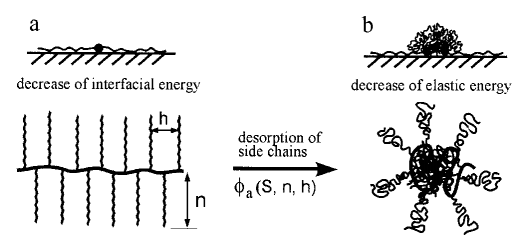
\includegraphics[scale=0.5]{./figures/1.png}
\caption{由侧链的部分解吸引起从棒状(a)到球状(b)的相变。所需的吸附侧链的分数$\phi _{a}$取决于铺展系数$S$、侧链的长度$n$和接枝密度$h^{-1}$。}
\end{figure}
1.尺度分析(Scaling Analysis)和理论背景在假定侧链部分脱附的情况下,对构象(1)随扩散系数的变化和(2)侧向压缩时的转变进行了理论分析。吸附刷在弱溶剂中的自由能$F$是由于界面能的平衡和弹性能的下降而产生的,而弹性能则是在解吸时降低的:
\begin{equation}
F=F_{el}^{2D}+F_{el}^{3D}+F_s+F_{mix}
\end{equation}
弹性力$p_s=f_sa/kT$和$p_b=f_ba/kT$表示归一化(无量纲)力,这两种力分别适用于侧链和脊骨的两端。吸附刷的弹性能$F_{el}^{2D}$是$p_s$和$p_b$作用力的结果:
\begin{equation}
\begin{aligned}
F_{el}^{2D}/kT & =N_{2D}n\left( p_s~coth~p_s-1-ln\frac{sinh p_s}{p_s} \right)	+N \left( p_b coth p_b-1-ln\frac{sinh p_b}{p_b} \right)\\
F_{el}^{3D}/kT & = N_{3D}r^2/na^2\\
\end{aligned}
\end{equation}
吸附刷的表面能取决于分子维数$L$、$R$和$r$
\begin{equation}
F_{s}=\gamma _{12}A_1+\gamma _1(A_0-A_1)+\gamma _2(A_2+A_1)cong ~const + \gamma_2Lr-SLR
\end{equation}
对自由能的最后贡献是侧链的混合熵:
\begin{equation}
\frac{F_{min}}{kT}=N_{2D}ln (N_{2D}/N)+N_{3D}ln(N_{3D}/N)
\end{equation}	
刷分子在单层中的总自由能可以表示为两个自变量的函数
\begin{equation}
\begin{aligned}
\frac{F}{kTN} & = \phi _an\left( p_s~coth~p_s-1-\ln\frac{sinh~p_s}{p_s} \right)+\left( p_b~coth~p_b-1-\ln\frac{sinh~p_b}{p_b} \right)\\
& +\frac{3(1-\phi_a)^2}{2x}+\gamma \sqrt{xn(1-\phi_a)}-Sn\phi_a+\phi_a\ln\phi_a+(1-\phi_a)\ln(1-\phi_a)\\
\end{aligned}
\end{equation}	
在扩展系数变化时的构象相变
\begin{figure}[H]
\centering
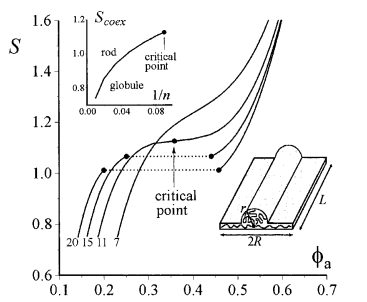
\includegraphics[scale=0.5]{./figures/11.png}
\caption{侧链长度n=7、11、15和20的侧链的扩散系数$S$与吸附侧链的分数之比。虚线显示出从球状到棒状的不连续相变。描述了两种构象与侧链长度共存时扩展系数$S_{coex}$的依赖关系。}
\end{figure}
侧向压缩下的构象相变\\
与变扩散系数下的相行为相似,侧链相对较短的分子其长度低于临界值,在侧向压缩作用下只表现为压力的逐渐增大。相反,具有较长侧链的刷分子在恒压下显示两种构象共存。在较低的压缩度下,人们观察到棒状构象,这相当于吸附侧链的更大一部分。在一定的表面压力下,观察到球状构象的出现,在此基础上发生了侧链的剧烈解吸。
\subsection{结论}
最后,观察到单个分子从棒状到球状构象的特殊转变。在恒压和恒温两种构象共存和分子构象标度分析的基础上,证明了这是一种一级相变。但有两个重要方面没有讨论到:(1)分子间相互作用和单层有序的影响;(2)二维刷的平衡构象。

	
\section{Elasticity-driven spontaneous curvature of a 2D comb-like polymer with repulsive interactions in the side chains(二维梳的弹性驱动自发曲率-如侧链中具有排斥作用的聚合物)}
\begin{center}
I.I. Potemkin\\
2003
\end{center}
\subsection{内容}
内容:本文以具有柔性、化学相同的侧链的二维梳状大分子为例,报道了弯曲过程中不同类型的不稳定性。证明,如果侧链单体单元间的相互作用是排斥的(好溶剂条件),如果侧链相对于主链可以翻转以达到自由能的最小值,那么梳的直线构象仅仅由于熵的原因向弯曲方向不稳定。
\begin{figure}[H]
\centering
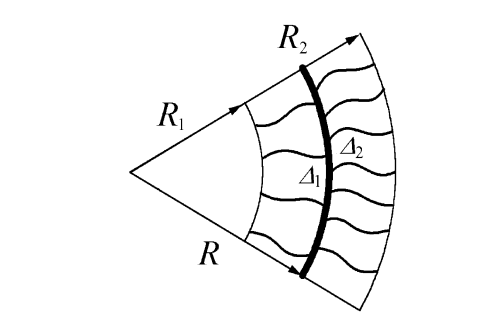
\includegraphics[scale=0.5]{./figures/2.png}
\caption{小段弯曲的2D梳子示意图。$R1$和$R2$是侧链的坐标凹部和凸部的端部,$R$是主干的曲率半径(梳)。侧链被均匀地接枝到主链上,距离$\Delta$是恒定的。凹面(左$\Delta_1=\Delta /\beta$)和凸面(右$\Delta_2=\Delta/(1-\beta)$)($\beta \leq 1/2$。}
\end{figure}
在平均场近似下,单元间相互作用的梳的单位长度自由能等于
\begin{equation}
F=F_{left}+F_{right}=N\left( \frac{Bv}{a} \right)^{2/3}\left[ \frac{1}{\Delta _1^{5/3}}\frac{P^{1/3}(z_1)W(z_1)}{K(z_1)}+\frac{1}{\Delta_2^{5/3}}\frac{P^{1/3}(z_2)W(z_2)}{K(z_2)} \right]
\end{equation}
这里$z_1=\phi(R)/\phi(R_1)\geq 1,z_2=\phi(R)/\phi(R_2)\geq 1$
\begin{figure}[H]
\centering
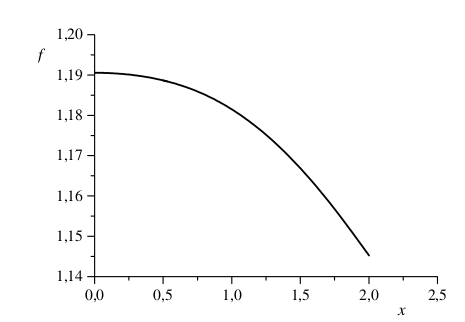
\includegraphics[scale=0.5]{./figures/12.png}
\caption{约化自由能$f=F\frac{\Delta}{N}\left( \frac{a\Delta}{vB} \right)^{2/3}$作为约化曲率$x=\frac{aN}{R}\left( \frac{vB}{a\Delta} \right)^{1/3}$的函数。}
\end{figure}
因此,梳子的自由能随弯曲而减小。这意味着梳子的直线构象在弯曲时是不稳定的,并伴随着侧链的重新分布。这种效应的物理解释:在对称梳的情况下,每条侧链被限制在一个矩形区域,从而导致链的均匀强拉伸。非对称梳子的侧链为圆形扇形,在梳子的凸侧,该区域的宽度从主干网区域增加到链的自由端区域。其结果是,局部链的拉伸远离了主链,导致链的总弹性能降低。由于侧链数量的减少,梳子凹侧链的拉伸也减小了。因此,梳子的不稳定性是由侧链的弹性驱动的。

本文证明了在侧链单体单元间排斥的情况下,即当线张力(三维物体表面张力的类似物)不存在时,伴随着侧链相对于主链的不均匀分布,二维分子梳的直线构象向弯曲方向是不稳定的。驱动力是侧
链的熵弹性。在脊椎骨的弯曲下,它们的伸长较少。

值得注意的是,所发展的平均场理论也可用于描述弯曲成圆柱的平面刷的双层结构。在这种情况下,参数$\Delta/2$应该具有每一层中每条链的平方的含义。虽然双层中的链比2D梳中的链拉伸要小,但双层的平面构象在弯曲进入圆柱体时也是不稳定的。然而,它也可以弯曲成一个球体。预测双层的最终形状需要额外的分析。


\section{Spontaneous Curvature of Comblike Polymers at a Flat Interface(梳状聚合物在平面界面上的自发曲率)}
\begin{center}
Igor I. Potemkin, Alexei R. Khokhlov†, Svetlana Prokhorova, Sergei S. Sheiko, Martin Möller, Kathryn L. Beer, and Krzysztof Matyjaszewski \\
2004
\end{center}
\subsection{内容}
用扫描力显微镜观察了吸附在平板基片上的分子刷的自发曲率。在强吸附条件下,对分子刷的二维模型进行了理论分析。虽然所有的侧链都被限制在基板平面上,但它们可以翻转并改变它们相对于主干网的位置。直链的不稳定性完全是由侧链的熵弹性引起的:侧链相对于主链的分布不均匀而得到较小的伸长。平衡,例如自发的曲率,是由侧链的弹性与稳定因素(如主链的固有刚度、侧链的混合熵,但刷的远部的体积相互作用除外)之间的竞争引起的。曲率半径与侧链聚合度成正比。讨论了侧链的多分散性的影响。
\subsection{吸附型梳状聚合物的模型与自由能}
刷分子在致密单层中每单位长度的自由能包括侧链和主链的弹性能以及侧链的混合熵
\begin{equation}
f=f_{left}+f_{right}+f_{bb}+f_{mix}
\end{equation}
\begin{figure}[H]
\centering
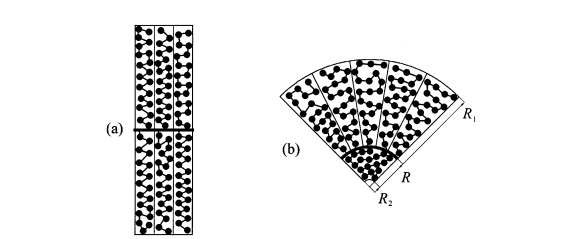
\includegraphics[scale=0.7]{./figures/3.png}
\caption{}
\end{figure}
我们将毛刷划分为主干中含有$dN$单体单元的部分,其中$dN _1$(左)和$dN_2$(右)侧链分别形成该截面的凸边和凹边。$dN \gg 1,dN_1>dN_2,dN_1+dN_2)=dN$。让我们将笔刷(脊骨)部分的曲率半径表示为$R$。形成笔刷凸边的侧链的弹性自由能可写为
\begin{equation}
\frac{\mathfrak{F}_{left}}{K_BT}=\frac{dN_1}{2\lambda _s}\int _{R}^{R_1} E(r)dr
\end{equation}
其中,$\lambda _s$是假定为柔性的侧链的Kuhn段长度,$\lambda _s \ll aM$。
\begin{equation}
\begin{aligned}
f_{left} & =\frac{d\mathfrak{F}_{left}}{dN~aK_BT}=\frac{\beta ^2R}{2\lambda _sa}\ln \left( \frac{R_1}{R} \right)=\frac{\beta^2R}{4\lambda_sa}\ln\left( 1+\frac{2aM\beta}{R} \right)	\\
f_{right} & =-\frac{(1-\beta)^2R}{4\lambda_sa}\ln(1-\frac{2aM(1-\beta)}{R})\\
f_{bb} &=\frac{\lambda _b}{2R^2}\\
f_{mix} & =\frac{1}{a}\left[ \beta\ln\beta +(1-\beta)\ln(1-\beta) \right]
\end{aligned}
\end{equation}	
假设刷分子达到平衡状态,意味着刷分子的总自由能应以$\beta$和$R$为函数。我们考虑刷的每一个碎片的小弯曲,伴随着平衡的侧链左右分布。在这种情况下,分子远的部分的相互作用不影响曲率半径。
\begin{equation}
\Delta f=f-\left[ \frac{M}{8\lambda _s}-\frac{\ln 2}{a} \right]	=z^2\left( \frac{2}{a}+\frac{18\lambda _b}{a^2M^2} \right)-\frac{3M}{5\lambda _s}z^4+...
\end{equation}	
\begin{figure}[H]
\centering
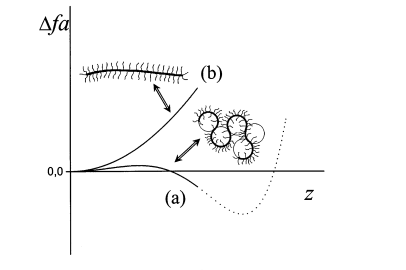
\includegraphics[scale=0.7]{./figures/13.png}
\caption{不同长度(或侧链长度)的毛刷$\Delta fa$的弯曲自由能随曲率$z$的变化特征:分别在$\lambda$的小值和高值下,刷段的弯曲(a)和直线(b)形状的稳定性}
\end{figure}
因此,本文讨论的柔性侧链聚合物的侧链长度与构象行为无关,分别由侧链和主链的熵弹性和弯曲弹性的竞争决定。


\section{Persistence Length of Comblike Polymers Strongly Adsorbed on a Flat Surface(梳状聚合物在平板表面强吸附的持久性长度)}
\begin{center}
Igor I. Potemkin\\
June 2. 2006
\end{center}
\subsection{内容}
本文主要对高分子的持久度$\lambda$对侧链段数的依赖提出了一个将理论和实验结合在一起的模型。证明了吸附的刷分子的持久长度对侧链的长度有较强的依赖性。持久长度受吸附侧链分数的控制:分数越高,持久长度越大。将吸附侧链的分数作为拟合参数,与实验数据进行了定量比较。
\begin{figure}[H]
\centering
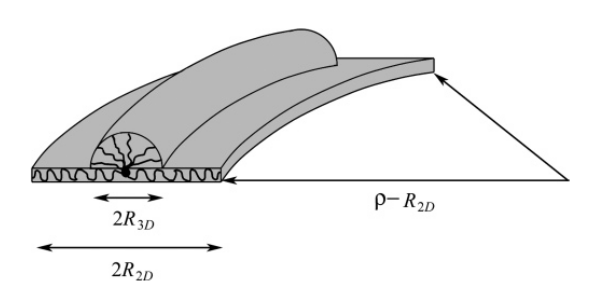
\includegraphics[scale=0.5]{./figures/4.png}
\caption{刷分子在平面上强烈吸附的示意图表示。}
\end{figure}
吸附刷的总持续长度为
\begin{equation}
\lambda=\lambda_{2D}+\lambda{3D}\approx n^3\left( \frac{\phi}{x} \right)^5\alpha +n\left( \frac{1-\phi}{x} \right)^3\alpha
\end{equation}		
经实验得,$\lambda \approx n^{v}\alpha,2\leq v \leq 3$,且$v\approx 3+5\ln \phi / \ln n+(1+\phi)^3/(\phi ^5 n^2 \ln n)+...,n\gg 1$。


\section{Block Copolymer Based Molecular Motor}
\begin{center}
Oleg E. Perelstein, Viktor A. Ivanov, Yury S. Velichko, Pavel G. Khalatur,Alexei R. Khokhlov, Igor I. Potemkin*\\
2007
\end{center}
\subsection{内容}
提出了一种基于二嵌段共聚物在图案表面强吸附的分子马达模型。即证明了由‘简单’单体单元组成的单个二嵌段共聚物链能够在结构固体表面上进行定向再吸附运动。
\begin{figure}[H]
\centering
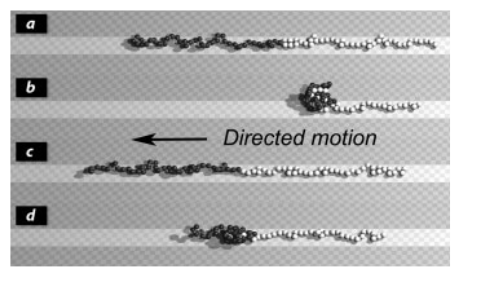
\includegraphics[scale=0.5]{./figures/5.png}
\caption{表面的深灰色区域对于单体单元的吸附是“禁止的”,只能沿着亮灰色的条纹发爬行。块A(黑色)受外场的周期性作用,导致周期性塌陷-再吸收循环。B块(白色)总是被吸附。链的位置显示在不同时刻:$t_a<t_b<t_c<t_d$。}
\end{figure}
嵌段共聚物分子通过以下方法进行模拟:用带FENE键相互作用势和单体-单体相互作用的Morse势的珠弹簧模型。

最后,我们用LD技术证明,强吸附的、组合对称的二嵌段共聚物的时间周期崩塌-再吸附可以诱导分子的定向运动(反应)。运动的轨迹是由表面的一个图案决定的。运动方向性的物理原因是摩擦力的各向异性。共聚物简化珠弹簧模型的数值计算结果与计算机模拟结果吻合较好。


\section{Nanopattern of Diblock Copolymers Selectively Adsorbed on a Plane Surface(两嵌段共聚物在平面选择性吸附的纳米形态)}
\begin{center}
I. I. Potemkin, E. Yu. Kramarenko,  A. R. Khokhlov,  R. G. Winkler, P. Reineker, P. Eibeck, J. P. Spatz, and M. Möller \\
1999
\end{center}
\subsection{内容}
在强分离极限条件下,研究了表面相互作用控制的微相分离导致A-B两嵌段共聚物在干超薄膜上形成化学非均匀表面纳米颗粒。在平面上,一个块体(A块)被强吸附,形成一个紧密结合的单分子层(二维熔体)。非吸附B块由于与基体上的A块层和空气不相容而聚集。因此,一种化学上不均匀的表面就会出现。根据嵌段长度比和相互作用参数,去湿的B块可以组装成球形表面胶束或蠕虫状表面聚集体,即点状或条纹状表面。
\begin{figure}[H]
\centering
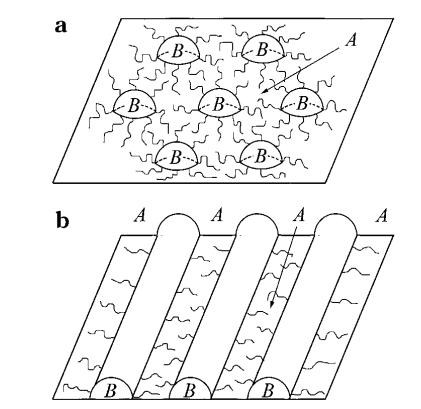
\includegraphics[scale=0.5]{./figures/8.png}
\caption{具有对平面强吸附的A块的A-B两嵌段共聚物在平面表面强吸附形成的模型表面胶束(a)和表面条纹(b)的示意图}
\end{figure}
值得注意的是,在水/空气界面具有一个疏水和一个聚电解质或极性嵌段的二嵌段共聚物体系中也观察到了多种形态的结构。特别是随着疏水和亲水块长度之比的增加,出现表面胶束、条纹和平面刷状结构。这些观测结果与我们的理论预测有很好的定性关系。

	
\section{Microphase Separation in Ultrathin Films of Diblock Copolymers with Variable Stickiness of One of the Blocks to the Surface(一种对表面的粘着性可变的两嵌段共聚物在超薄薄膜上的微相分离)}
\begin{center}
Igor I. Potemkin and Martin Möller \\
2005
\end{center}
\subsection{内容}
在强隔离极限条件下,从理论上研究了表面相互作用控制的微相分离导致A-B两嵌段共聚物在干超薄膜中上形成化学非均匀表面纳米颗粒。在平面上,其中一个块体(A块)被强吸附,形成一个紧密结合的单分子层(二维熔体)。第二块(B块)与表面的相互作用可以从强吸引(二维构象)到强斥力(三维构象)变化,包括弱相互作用机制。由于A、B单体单元具有很强的不相容性,会出现化学不均匀的表面形态。根据块体长度比和相互作用参数,可以形成不同的微结构。它们由表面胶束组成,表面胶束具有突出或扁平的圆盘状核,平行条纹,以及单体厚芯和突出电晕(反盘状结构)的孔状胶束。得到了这类结构的几何参数与块体长度的关系。该理论最重要的预测是,其中一个块的粘着性的变化会导致形态的变化。
\begin{figure}[H]
\centering
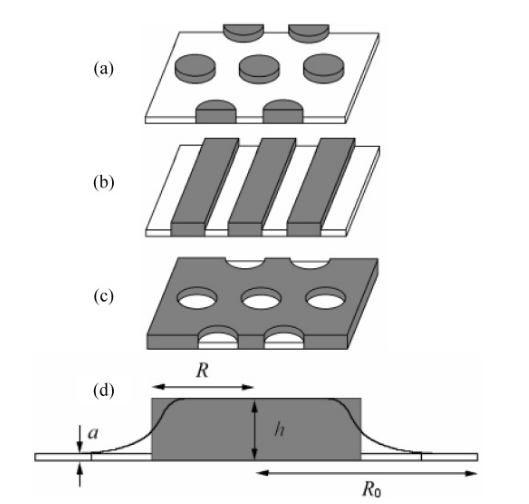
\includegraphics[scale=0.5]{./figures/7.png}
\caption{A-B两嵌段共聚物与强吸附A嵌段(白色)和部分解吸B嵌段(灰色)形成的微结构示意图表示:(a)六边形晶格对称排列的盘状胶束;(b)平行条纹;(c)六角形晶格(反盘状胶束)对称排列的孔。(d)B块的核心的平滑轮廓被建模为阶梯式形状。}
\end{figure}
\textbf{盘状}\\
生成的非聚集链的自由能可以写成
\begin{equation}
F_{homo} =
\begin{cases}
-\frac{3N_BS_B^2}{8\pi ^2}+4\pi\sqrt{\frac{\pi N_B}{3S_B}}\left( \bar{r}_{Ba}+(\bar{r}_{AB}-\bar{r}_{ba})\frac{3S_B}{4\pi ^2} \right), & S_B\leq\frac{4\pi^2}{3} \\
-N_B\left( S_B-\frac{2\pi ^2}{3} \right)+2\sqrt{\pi N_B}\bar{r}_{AB}, & S_B>\frac{4\pi^2}{3}
\end{cases}
\end{equation}
\begin{figure}[H]
\centering
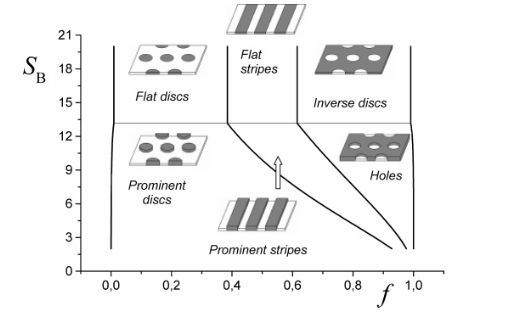
\includegraphics[scale=0.5]{./figures/14.png}
\caption{B单体单元的分数$f=N_B(N_A+N_B)$的薄膜的相图和扩展参数$S_B$有关。水平线$S_B=4\phi^2/3$分裂平面区和突出区。为保证A块的二维构象,扩展参数$S_A$满足不等式$S_A \geq 4\pi^2/3$}
\end{figure}

\section{Nanostructured Ultrathin Films Obtained by the Spreading of Diblock Copolymers on a Surface(表面上的两嵌段共聚物通过扩散制备纳米结构超薄薄膜)}
\begin{center}
Elena S. Patyukova  and Igor I. Potemkin\\
2007
\end{center}
\subsection{结论}
本文提出了一种将A-B两嵌段共聚物在表面进行扩散而超薄薄膜中形成纳米粒子的理论。A块在基体上被强吸附(扩散),吸附强度可以变化。B块与基片不兼容,但它们可以在A块的层上传播。我们预测六边形对称的圆盘状胶束和平行的条状胶束和双层胶束是稳定的.结果的结构类型及其几何参数取决于共聚物的组成和相互作用参数。我们将这些结果与两个块在衬底上的扩展情况下得到的结果联系起来,并构造了一个统一的相图。
\begin{figure}[H]
\centering
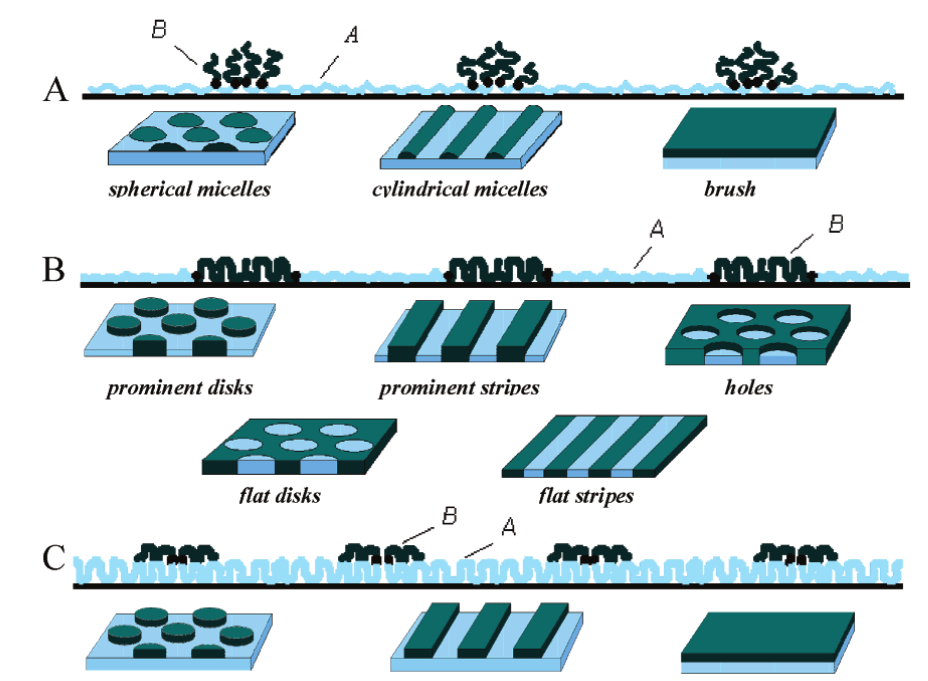
\includegraphics[scale=0.4]{./figures/6.png}
\caption{三种超薄两嵌段共聚物薄膜的原理图表示:(a)A嵌段在基体上吸附强烈,而B嵌段既不与基体相容,也与A嵌段层不相容。(b)两个区块都被吸附在基片上。(c)A嵌段在基底上吸附块(吸附程度不同)。B块与基片不兼容,但它们可以在A块的层上传播。}
\end{figure}
结果表明,薄膜的形貌受二嵌段共聚物的组成和A块对基片的吸引强度和B块对A层的吸引强度控制。计算得到的薄膜结构包括圆盘状、带状和双层结构。


\textbf{引用}

\section{Microphase Separation Induced by Complexation of Ionic−Non-Ionic Diblock Copolymers with Oppositely Charged Linear Chains(离子-非离子双嵌段共聚物带电的线性链络合引起的微相分离)}
\begin{center}
Anna S. Bodrova,Elena Yu. Kramarenko, and Igor I. Potemkin\\
2009
\end{center}
\subsection{内容}
本文发展了一种微相分离理论,它是由带电(A)和中性(B)嵌段组成的柔性AB嵌段共聚物通过静电作用与相对带电的线性链(C)络合而形成的溶液沉淀。分析了选择性溶剂的存在方式:A段和C链组分的溶剂为Θ,而B段的溶剂含量较低。尽管有选择性,但化学计量配合物由于涨落引起的静电吸引而沉淀。根据二嵌段共聚物的组成、溶剂的选择性和荷电基团的分数,正、反球形、柱状和层状结构在沉淀剂中是稳定的。在强偏析近似下构造相图。预测了溶剂质量和荷电基团分数变化引起的形态转变。
\begin{figure}[H]
\centering
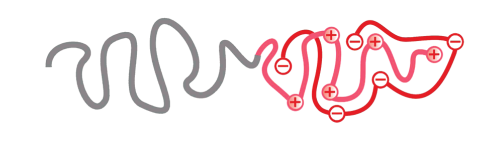
\includegraphics[scale=0.4]{./figures/9.png}
\caption{含非离子和离子的二嵌段共聚物的图。带相反电荷的线性链块}
\end{figure}
	
\begin{figure}[H]
\centering
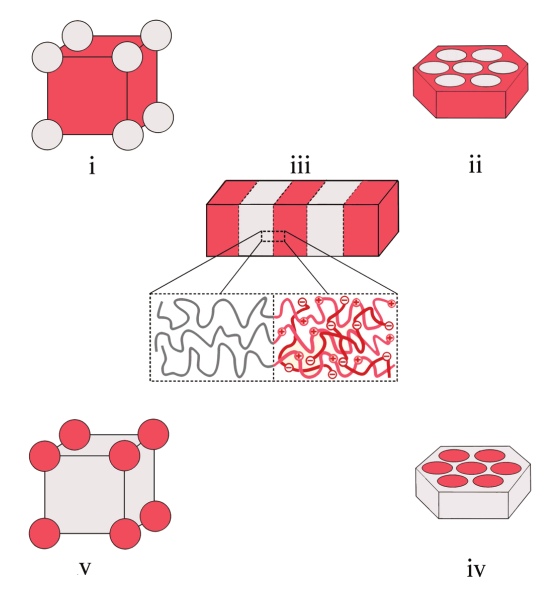
\includegraphics[scale=0.4]{./figures/10.png}
\caption{(i)非离子(B)和(v)离子(A+C)核填充BCC球形胶束,(ii)非离子和(iv)离子核填充六方圆柱胶束,(iii)层状结构。}
\end{figure}
本文发展了AB嵌段共聚物和线性链溶液中微相分离的强偏析理论。共聚物的(A)嵌段带电,中性嵌段(B)中等不溶(由B块形成的球状畴可以包含溶剂的某些部分)。带相反电荷的线性链(C)与A块形成化学计量配合物。在半稀溶液中,络合的两嵌段共聚物和线型链由于吸引的波动引起静电相互作用而沉淀。B与A+C的不相容性导致沉淀剂的结构。我们预测了(i)非离子(B)和(ii)离子(A+C)核的BCC填充球形胶束的热力学稳定性,(iii)非离子和(iv)离子核的六方填充圆柱胶束和(v)层状结构的球形胶束的热力学稳定性。建立了微相分离的相图。在弱聚电解质的情况下,pH值和溶剂质量的变化都会引起形态转变。


\section{Floated Lamella Films of Styrenic Block Copolymers: Local Shearing Deformations and Heterogeneous Layer at the Substrate(苯乙烯嵌段共聚物的浮片膜:局部剪切变形和基片上的非均质层)}
\begin{center}
Eva Max,  Markus Hund, Igor I. Potemkin,and Larisa Tsarkova\\
2013
\end{center}
\subsection{内容}
研究了热平衡嵌段共聚物薄膜的自由表面和基片−薄膜界面,形成了玻璃状−胶状层,并对形成的薄膜厚度进行了量化。除了揭示在约束条件下纳米结构聚合物薄膜的自适应力学行为外,本文报道的观测结果还可用于设计叠加的地形结构,方法是控制衬底上的润湿,并能更好地预测化学图案表面的结构形成和模式转移的可能机制。

\section{Effect of Architecture on Micelle Formation and Liquid-Crystalline Ordering in Solutions of Block Copolymers Comprising Flexible and Rigid Blocks: Rod–Coil vs Y-Shaped vs Comblike Copolymers(结构对柔性和刚性嵌段共聚物溶液中胶束形成和液晶有序性的影响:棒状−线圈vsY型共聚物vs梳状共聚物
)}
\begin{center}
Kirill E. Polovnikov , and Igor I. Potemkin\\
October 6, 2017
\end{center}
\subsection{内容}
采用耗散粒子动力学(DPD)模拟方法,研究了两亲性嵌段共聚物在选择性溶剂中的胶束形成。比较了Y形(不溶性刚性块和两个柔性可溶臂)和梳状(不溶性刚性侧链可溶骨架)共聚物与等效棒型−线圈双嵌段共聚物的自组装特性。但是两亲梳状大分子形成胶束以及侧链刚性对内胶束结构的影响尚未得到研究
\begin{figure}[H]
\centering
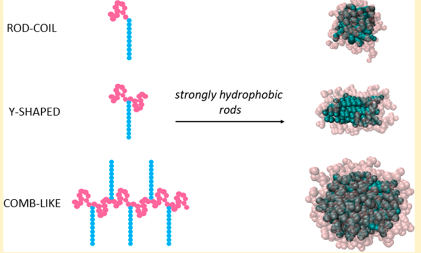
\includegraphics[scale=0.4]{./figures/15.png}
\caption{}
\end{figure}
本文研究了溶液中的胶束形成,具有柔性和杆状的两亲性大分子使用耗散粒子动力学的块。比较了不同的结构:不同长度的棒状−线圈双嵌段共聚物、Y型共聚物和梳状共聚物。考虑了一种选择性溶剂,它对柔性块有利,对刚性块不利。因此,刚性块体聚集到胶束的核心是伴随着它们的向列有序。具有柔性主链和棒状侧链的块状梳状大分子,如果相邻侧链之间间隔的长度等于杆的长度,则形成近球形胶束。相反,更紧密的棒状−线圈双嵌段和Y形大分子形成了较小的胶束,其核心具有更好的向列有序性。即使在溶剂选择性很高的条件下,核内棒的向列有序性也是相当弱的。物理原因是,由于电晕中的环的密集堆积造成的,主链连接的棒,其液晶有序伴随着自由能的惩罚。相反,更紧密的棒状−线圈双嵌段和Y形大分子形成了较小的胶束,其核心具有更好的向列有序性。
\begin{figure}[H]
\centering
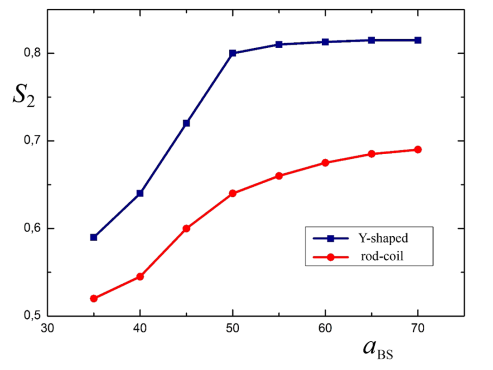
\includegraphics[scale=0.4]{./figures/16.png}
\caption{胶束的向列序参数$S_2$与棒状块体溶剂质量的关系}
\end{figure}
\begin{figure}[H]
\centering
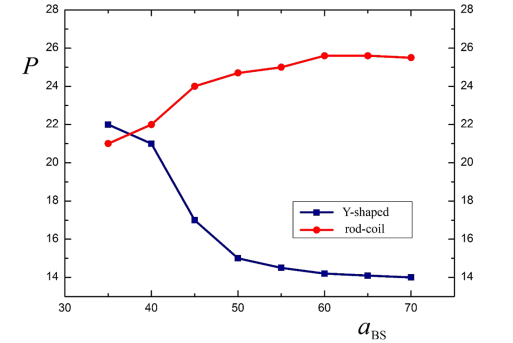
\includegraphics[scale=0.4]{./figures/17.png}
\caption{胶束的聚集数P与棒状块体溶剂质量的关系}
\end{figure}
由于溶剂质量(温度)的变化引起的Y型共聚物胶束的向列序参数和聚集数的急剧变化,可能在许多传感器的应用中得到应用。同时,有趣的是,梳状结构负责形成具有弱有序向列相核心的球形胶束,这些胶束在外部条件(如温度)的变化下是非常稳定的,从而导致溶剂质量的变化。这一事实在许多应用中可能是有用的,在这些应用中,稳定的液晶有序是非常重要的。


\section{Amphiphilic Arborescent Copolymers and Microgels: From Unimolecular Micelles in a Selective Solvent to the Stable Monolayers of Variable Density and Nanostructure at a Liquid Interface}	
\begin{center}
Rustam A. Gumerov, Andrey A. Rudov, Walter Richtering, §Martin Moller, and Igor I. Potemkin\\
April 10, 2017
\end{center}
\subsection{内容}
在选择性溶剂和液体界面上,通过耗散粒子动力学(DPD)模拟,研究了两代(G2和G3)的两亲性树形嵌段共聚物和通过两嵌段共聚物交联得到的聚合物微凝胶。单分子在液体(油、水)界面上的吸附导致两亲性基团的平坦和偏析:亲水和疏水基团分别暴露于水和油中。根据单体单元间相互作用的特点,单体单元之间的相互作用可以由温度或溶剂质量控制,在大分子中可以形成Janus、片状结构和纳米隔离结构。它们在界面上的自组装会导致松散和致密的单分子层的形成,这种单层可以是均匀的,也可以是纳米结构的。G2大分子的快速吸附动力学使其成为乳液的有效稳定剂。

\begin{figure}[H]
\centering
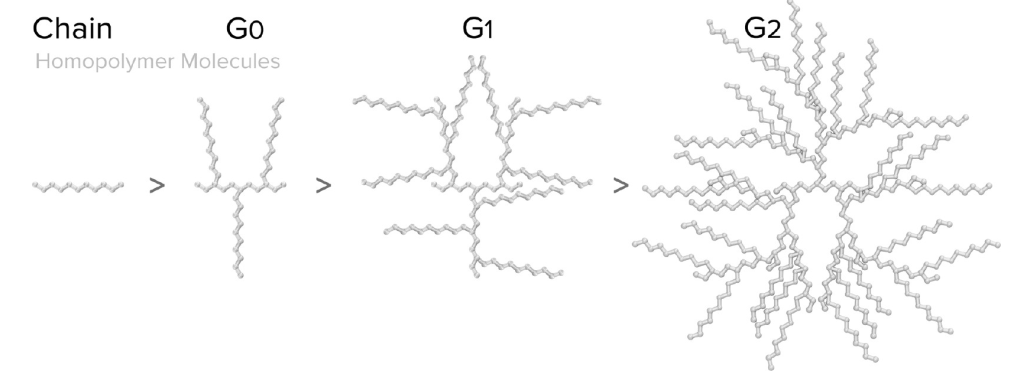
\includegraphics[scale=0.4]{./figures/19.png}
\caption{}
\end{figure}

\begin{figure}[H]
\centering
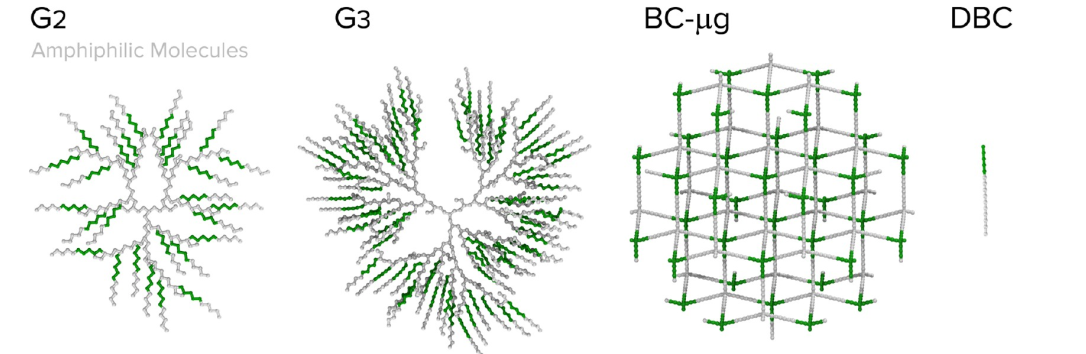
\includegraphics[scale=0.4]{./figures/20.png}
\caption{G2和G3树枝状共聚物、嵌段共聚物微凝胶、BC-μG和线型二嵌段共聚物的一级结构。灰珠对应A(表面上亲水性)区块,绿色对应B(表面上疏水)区块。}
\end{figure}
本论文的目的是通过计算机模拟对树枝状共聚物进行比较研究。我们分析了不同代的单枝大分子在选择性溶剂中的构象,并研究了它们的自组装与通过二嵌段共聚物交联形成的等效二嵌段共聚物和微凝胶的对比。然后研究了单树枝状分子吸附在两种不相容液体界面上的构象及其面内自组装。最后比较了树枝状共聚物与线型二嵌段共聚物和分子量相近的嵌段共聚物微凝胶的稳定性。
\begin{figure}[H]
\centering
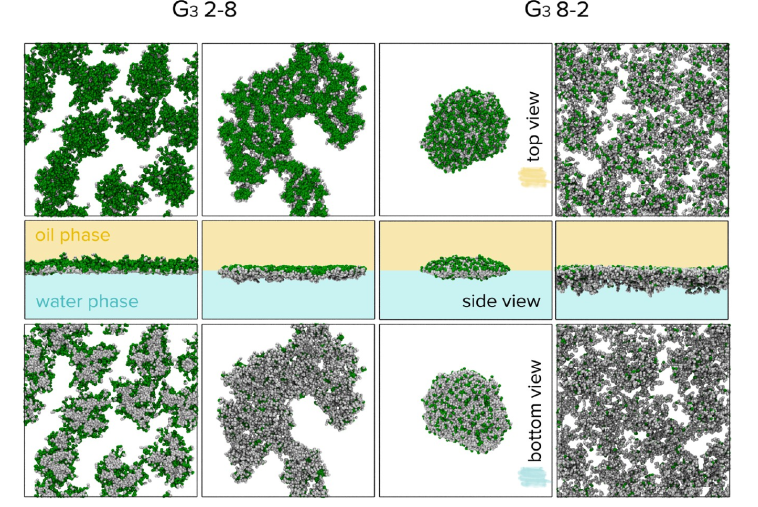
\includegraphics[scale=0.4]{./figures/21.png}
\caption{树枝状G3共聚物具有强不对称二嵌段组成的液体界面模拟快照:$A_2B_8$(左两柱)和$A_8B_2$(右两柱)。第一列和第三列分别展示了A和B珠之间的相互吸引和排斥机制。第二列和第四列代表相反的制度。}
\end{figure}

\begin{figure}[H]
\centering
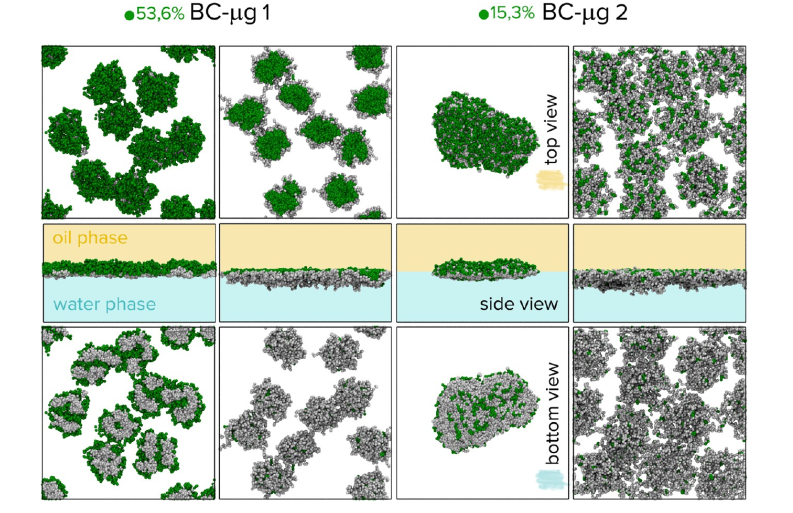
\includegraphics[scale=0.4]{./figures/22.png}
\caption{$μG-53.6\%$(左两柱)和$μG-15.3\%$(右两柱)组成强烈不对称的嵌段共聚物微凝胶覆盖液体界面的模拟快照。这些数字代表绿色珠子的总分数。}
\end{figure}		

	
\section{Self-assembly of rarely polymer-grafted nanoparticles in dilute
solutions and on a surface: From non-spherical vesicles to graphene-
like sheets(少量聚合物接枝纳米粒子在稀溶液和表面上的自组装:从非球形小泡到石墨烯样片)}
\begin{center}
Vitaly S. Kravchenko , Igor I. Potemkin\\
12 March 2018
\end{center}
\subsection{内容}
聚合物接枝纳米粒子能够自组装成稳定的不同形貌的纳米结构。组装的驱动力是纳米粒子的短程吸引力和接枝链的远程排斥之间的竞争。研究了纳米粒子的溶剂质量、接枝密度和链长的影响。我们已经证明,类似于单晶的非球形小泡在稀溶液中是稳定的。在它们中,壁代表一片六方填充的纳米粒子,这些纳米粒子急剧弯曲成为封闭的形成面和边缘。溶剂质量的提高导致了一系列的转变:囊泡-管-穿孔板-线程。纳米粒子在反溶剂表面的吸附会导致其二维自组装。我们预测了纳米粒子在六方网络中的有序性,这与石墨烯的结构类似。建立了二维和三维状态的示意图。\\
\begin{figure}[H]
\centering
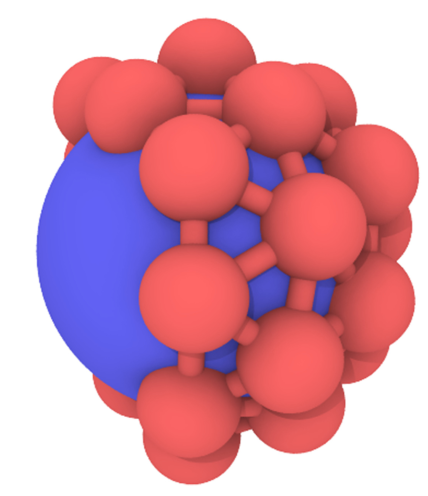
\includegraphics[scale=0.4]{./figures/23.png}
\caption{纳米粒子示意图}
\end{figure}
\begin{figure}[H]
\centering
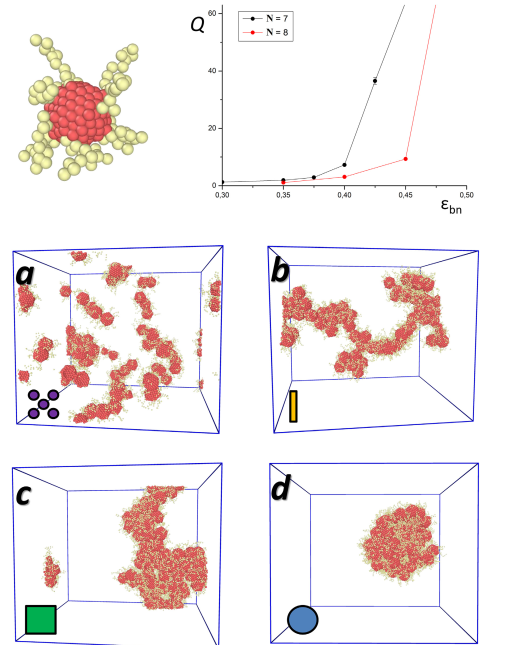
\includegraphics[scale=0.4]{./figures/24.png}
\caption{上行是$n=12$时的接枝链的单纳米粒子。自组装纳米结构在不同接枝链长度($N=7$(黑)、$8$(红)和固定$n=12$的平均聚集数Q随相互作用参数$\varepsilon_{bn}$的变化而变化。中行和下行是自组装纳米结构,系列I,$N= 8,n=12$,在相互作用参数$\varepsilon_{bn}$的不同值下得到:$\varepsilon_{bN}=0.4\varepsilon(a),0.475\varepsilon(b),0.55\varepsilon(c),0.65\varepsilon(d)$。}
\end{figure}













%3.Structure of Bottle Brush Polymers on Surfaces: Weak versus Strong Adsorption


%4.Hybrid Core-Shell (HyCoS) Nanoparticles produced by Complex Coacervation for Multimodal Applications


%5.Bimodal probability density characterizes the elastic behavior of a semiflexible polymer in 2D under compression
	


%1.Individual bottle brush molecules in dense 2D layers restoring high degree of extension after collapse-decollapse cycle: Directly measured scaling exponent (密集2D层中单个瓶刷分子恢复崩塌-脱粘循环后的高度伸展-直接测量的比例指数)

%作者:M. O. GallyamovEmail authorB. TartschI. I. PotemkinH. G. BörnerK. MatyjaszewskiA. R. KhokhlovM. Möller 时间:2009年










\cite{tam19912d}
%\bibliography{../ref}
\end{document}
